\chapter{Técnicas de Diseño de Algoritmos}

\section{Complejidad}

\subsection{Repaso de complejidad computacional}

La complejidad computacional es una técnica de análisis de algoritmos, en particular, de su tiempo de ejecución. Es de carácter \textit{teórico}: se basa en determinar matemáticamente la cantidad de operaciones que llevará a cabo el algoritmo para una instancia de tamaño dado, indendientemente de la máquina sobre la cuál se implementa y el lenguaje utilizado.

\subsubsection{Definición informal}

La complejidad de un algoritmo es una función $T_A: \N \longrightarrow \R_{>0}$ que representa el tiempo de ejecución en función del tamaño de la entrada. Para distinguir entre entradas de un mismo tamaño, se pueden considerar:
\begin{itemize}
    \item \textbf{Complejidad de peor caso}:\footnote{$t_A: I_A \longrightarrow \R_{>0}$ devuelve el tiempo de ejecución para una instancia particular del problema $A$.}
          $$T_{\text{peor}}(n) = \max{\{t_A(i)} \mid I \in I_A, |I| = n\}$$
    \item \textbf{Complejidad de mejor caso}:
          $$T_{\text{mejor}}(n) = \min{\{t_A(i)} \mid I \in I_A, |I| = n\}$$
    \item \textbf{Complejidad de caso promedio}:\footnote{$P(I)$ es la probabilidad de que la entrada sea la instancia $I$.}
          $$T_{\text{prom}}(n) = \sum_{I \in I_A, |I| = n} P(I) \cdot t_A(I) $$
\end{itemize}

Para ciertos algoritmos, conviene hacer un análisis más profundo que distingue entre tipos de instancias particulares al problema.

Estas definiciones no son rigurosas: no contienen ninguna indicación sobre cómo determinar $T_A$ para un algoritmo $A$, y el ``tiempo de ejecución'' ni siquiera tiene unidades de medida. Para formalizarlas, es necesario definir un \textit{modelo de cómputo}.

\subsubsection{Modelo de cómputo: Máquina RAM}
\label{maquina-ram}

La \textit{Máquina RAM} es una máquina abstracta que funciona como modelo de cómputo. Nos permite modelar computadoras en las que la memoria es suficiente y los enteros involucrados en los cálculos entran en una palabra\footnote{Una \textit{palabra} es el tamaño de una celda de memoria}. Este modelo cuenta con:
\begin{itemize}
    \item \textbf{Memoria Principal}: Una sucesión de celdas numeradas (tantas como se necesiten). Cada una puede guardar un entero de tamaño arbitrario.
    \item \textbf{Registro Acumulador}: un registro especiel se usa como (generalmente primer) operando en las operaciones.
    \item \textbf{Acceso Aleatorio}: Acceso directo a cualquier celda en tiempo constante. También cuenta con direccionamiento indirecto: la dirección accedida puede ser el valor de una celda (un \textit{puntero}).
    \item \textbf{Programa}: Se codifica en una serie de instrucciones, y se almacena en una memoria aparte de la principal. Hay un \textit{contador de programa}, que identifica la próxima a ser ejecutada y puede ser manipulado a través de ciertas instrucciones (\textit{jumps}).
\end{itemize}

Tanto la entrada como la salida son representadas como una sucesión de celdas numeradas, cada una con un entero de tamaño arbitrario. Para codificar un programa, es necesario definir un \textit{set de instrucciones}. Un ejemplo posible sería el siguiente\footnote{Este ejemplo no es de ninguna forma minimal, pero es similar a un set de instrucciones RISC para una computadora real.}:
\begin{itemize}
    \item \textsc{Load} \code{valor} -- Carga un valor en el acumulador.
    \item \textsc{Store} \code{valor} -- Carga el acumulador en un registro.
    \item \textsc{Add} \code{valor} --Suma el operando al acumulador
    \item \textsc{Sub} \code{valor} -- Resta el operando al acumulador
    \item \textsc{Mult} \code{valor} -- Multiplica el operando por el acumulador
    \item \textsc{Div} \code{valor} -- Divide el acumulador por el operando
    \item \textsc{Read} \code{valor} -- Lee un nuevo dato de entrada → operando
    \item \textsc{Write} \code{valor} -- Escribe el operando a la salida
    \item \textsc{Jump} \code{label} -- Salto incondicional
    \item \textsc{Jgtz} \code{label} -- Salta si el acumulador es positivo
    \item \textsc{Jzero} \code{label} -- Salta si el acumulador es cero
    \item \textsc{Halt} -- Termina el programa
\end{itemize}

Para calcular la complejidad de un programa, se asume que cada instrucción tiene un tiempo de ejecución constante. En ese caso, se puede definir $t_A(I) = $ suma de los tiempos de ejecución de las instrucciones ejecutadas por el algoritmo $A$ para la instancia $I$. Esto es casi suficiente para calcular $T_A(n)$: solo resta definir $|I|$, el tamaño de la instacia.

\subsubsection{Modelo uniforme}

En este modelo, cada \textbf{dato individual} ocupa una celda de memoria, y cada operación básica tiene tiempo de ejecución constante. Esto resulta razonable cuando la entrada es una estructura de datos y cada dato entra en una palabra de memoria. Bajo esta suposición, el tamaño de entrada se define como la cantidad de datos individuales de la instancia.

Sin embargo, para algoritmos que operan sobre un entero particular, esta definición no resulta adecuada. Por ejemplo, se puede tomar el siguiente algoritmo, que determina si un número es o no primo:
\begin{codebox}
    \Procname{$\proc{Es-Primo}(n)$}
    \li \For $i \gets 2$ \To $\lceil\sqrt{n}\rceil$ \Do
    \li \If $n \equiv 0 \mod{i}$ \Then
    \li \Return \const{false}
    \End
    \End
    \li \Return \const{true}
\end{codebox}

Según la definición anterior, el tamaño de la entrada de $\proc{Es-Primo}$ es siempre $1$, lo cual es anti-intuitivo: sería conveniente poder definir la complejidad de este algoritmo en función del tamaño de $n$.

\subsubsection{Modelo logarítmico}

En este caso, el tamaño de la instancia se define como la cantidad de símbolos de un \textbf{alfabeto} necesaria para representarla, y el tiempo de ejecución de cada operación elemental depende del tamaño de los operandos (definido de la misma manera). Esto es apropiado para algoritmos que toman como input un número fijo de datos individuales.

Para representar los datos, se suele tomar como alfabeto $\mathbb{B} = \{0, 1\}$, los dígitos binarios. En tal caso, el tamaño de un entero $n \in \Z$ es $L(n) = \lceil\log_2{n}\rceil + 1$ bits, mientras que para almacenar una lista de $m$ enteros se necesitan $L(m) + mL(N)$, donde $N$ es el valor máximo posible en la lista.

\subsection{Notación O}

Para comparar tiempos de ejecución entre distintos algoritmos, es conveniente obviar constantes de proporcionalidad y enfocarse en el comportamiento asintótico de las complejidades. Con eso en mente, se definen las clases:
\begin{align*}
    f \in \BigO{g}     & \iff \exists c \in \R_{>0}, n_0 \in \N \mid \forall n \geq n_0,\ f(n) \leq c \cdot g(n) \\
    f \in \BigOmega{g} & \iff \exists c \in \R_{>0}, n_0 \in \N \mid \forall n \geq n_0,\ f(n) \geq c \cdot g(n) \\
    f \in \BigTheta{g} & \iff f \in \BigO{g} \land f \in \BigOmega{g}
\end{align*}

Informalmente, $f \in \BigO{g}$ implica que $f$ crece a lo sumo tan rápido como $g$.

\subsubsection{Complejidades comunes}

\begin{itemize}
    \item Si un algoritmo es\BigO{\log{n}}, se dice \textbf{logarítmico}.
    \item Si un algoritmo es\BigO{n}, se dice \textbf{lineal}.
    \item Si un algoritmo es\BigO{n^2}, se dice \textbf{cuadrático}.
    \item Si un algoritmo es\BigO{n^3}, se dice \textbf{cúbico}.
    \item Si un algoritmo es\BigO{n^k}, se dice \textbf{polinomial}.
    \item Si un algoritmo es $\BigO{k^n}\ (k > 1)$, se dice \textbf{exponencial}.
\end{itemize}

Además, se tiene:
\begin{align*}
    \BigO{n^k}     & \subsetneq \BigO{d^n}\ \forall k, d \in \N   \\
    \BigO{\log{n}} & \subsetneq \BigO{n^k}\ \forall k \in \R_{>0}
\end{align*}

\subsection{Problemas ``bien resueltos'' e intractabilidad}

Un problema se denomina \textit{bien resuelto} si existe un algoritmo de tiempo polinomial que lo resuelve. Esto se debe a que el tiempo de ejecución de los algoritmos exponenciales crece demasiado rápido: su ejecución puede resultar infactible para valores de $n$ pequeños.

\begin{figure}[H]
    \centering
    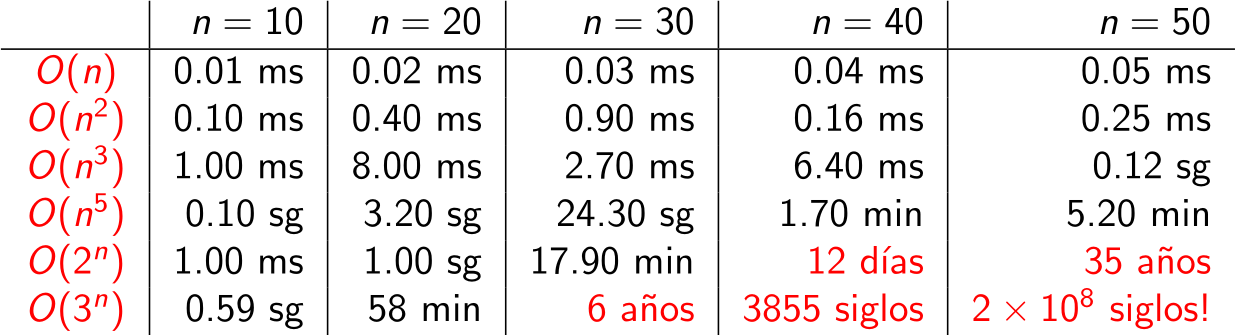
\includegraphics[width=0.7\textwidth]{tabla_complejidades.png}
    \caption*{Tabla de comparaciones de los posibles tiempos de ejecución para distintas clases de complejidad.}
\end{figure}

Sin embargo, cabe destacar que:
\begin{itemize}
    \item Si los tamaños de instancias no son muy grandes, un algoritmo exponencial puede ser apropiados.
    \item Un algoritmo puede ser polinomial, pero con un exponente o una constante demasiado grande para ser aplicado en la práctica.
    \item Existen ciertos algoritmos con complejidad de peor caso exponencial, pero que en la práctica son muy eficientes (como el método \textit{simplex}).
\end{itemize}

\section{Backtracking}

\subsection{Fuerza bruta}

Un algoritmo de \textit{fuerza bruta} (también llamado de \textit{búsqueda exhaustiva}) analiza todas las posibles configuraciones de la salida, hasta encontrar una que cumple con los requerimientos del problema.

\subsubsection{Ejemplo: Problema de las $n$ damas}

\begin{problema}
    Ubicar $n$ damas en un tablero de ajedrez de $n \times n$ casillas, de forma que ninguna dama amenace a otra.
\end{problema}

\begin{figure}[H]
    \centering
    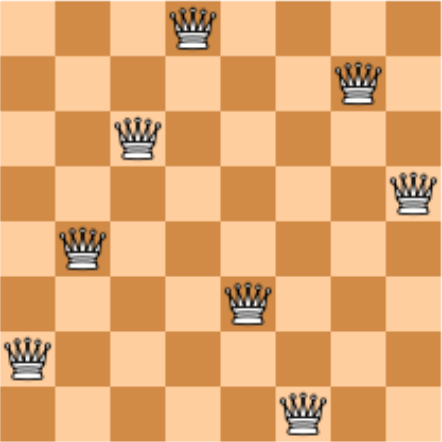
\includegraphics[width=0.3\textwidth]{solucion_n_damas.png}
    \caption*{Solución posible para el caso $n = 8$}
\end{figure}

Un posible algoritmo de fuerza bruta sería recorrer todos los posibles subconjuntos de $n$ casillas, verificando si algún par de reinas se amenaza en caso de ser ubicarlas en las casillas del subconjunto. Sin embargo, esto no es muy eficiente: para $n = 8$, implicaría recorrer $\binom{64}{8} = 4.426.165.368$ combinaciones.

Se pueden lograr mejoras aprovechando la estructura del problema: como cada columna debe tener exactamente $1$ dama, las configuraciones exploradas pueden representarse como un vector $(a_1, ..., a_n)$, con $a_i \in \{1, ..., n\}$ indicando la fila de la dama que está en la columna $i$. Además, cada fila tiene exactamente una reina, así que los elementos del vector no se repiten. Por ende, la cantidad de combinaciones se reduce a $n!$, que para el caso $n=8$ es $8! = 40.320$. No obstante, esto puede mejorarse.

\subsection{Backtracking}

El backtracking es una técnica general de diseño de algoritmos que consiste de extender las soluciones parciales $a = (a_1, ..., a_k), k < n$, agregando un elemento $a_{k+1}$ al final del mismo. Si se detecta que $S_{k+1}$, el conjunto de soluciones que tienen al vector como prefijo, es vacío, se retrocede a la solución anterior. Esto permite descartar configuraciones parciales apenas se determina que no pueden llevar a una solución. Los algoritmos de backtracking siguen el siguiente esquema general:
\begin{codebox}
    \Procname{$\proc{BT}(a)$}
    \li \If $\neg\proc{Es-Válida}(a)$ \Then
    \li \Return
    \End
    \li \If $\proc{Es-Solución}(a)$ \Then
    \li $\proc{Procesar}(a)$
    \li \Return
    \End
    \li \For $a' \in \proc{Sucesores}(a)$ \Do
    \li $\proc{BT}(a')$
    \End
\end{codebox}

Si solo se busca una solución, esto se puede volver más eficiente usando una variable global \id{encontr\acute{o}}:
\begin{codebox}
    \Procname{$\proc{BT}(a)$}
    \li \If $\neg\proc{Es-Válida}(a)$ \Then
    \li \Return
    \End
    \li \If $\proc{Es-Solución}(a)$ \Then
    \li $\id{sol} \gets a$
    \li $\id{encontr\acute{o}} \gets \const{true}$
    \li \Return
    \End
    \li \For $a' \in \proc{Sucesores}(a)$ \Do
    \li $\proc{BT}(a')$
    \li \If $\id{encontr\acute{o}}$ \Then
    \li \Return
    \End
    \End
\end{codebox}

Para que el backtracking sea eficiente, el procedimiento \proc{Es-Válida} debe ser capaz de identificar algún conjunto de instancias inválidas, y no puede tener una complejidad demasiado grande.

En el problema de las $n$ damas, se puede chequear en cada paso si alguna reina amenaza a la recién agregada. Esto se puede realizar en tiempo lineal, y por la construcción de las soluciones solo hace falta comprobar las amenazas diagonales. Utilizando este algoritmo, cualquier configuración de $n$ elementos que no haya sido rechazada es una solución válida.

\subsubsection{Ejemplo: Resolución de Sudokus}

\begin{problema}
    Encontrar una asignación de números a casillas que resuelve un Sudoku particular.
\end{problema}

\begin{figure}[H]
    \centering
    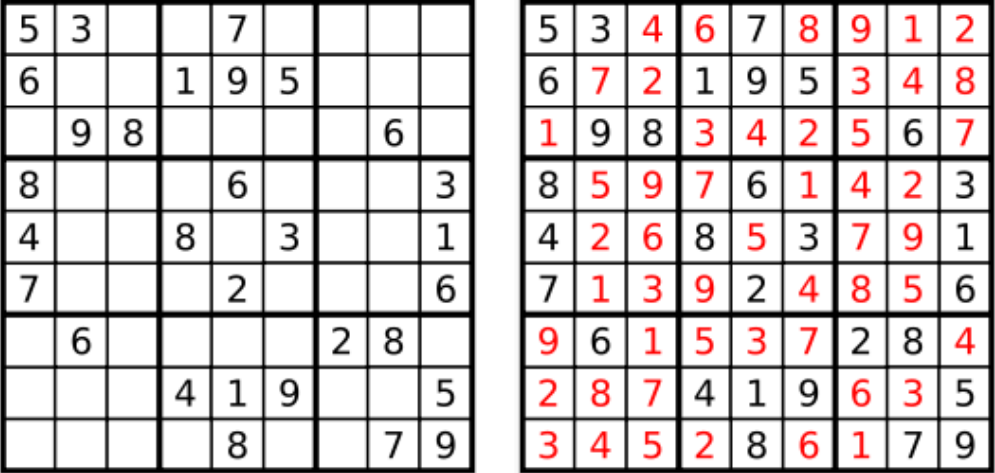
\includegraphics[width=0.8\textwidth]{sudoku.png}
    \caption*{Ejemplo de un Sudoku y su solución.}
\end{figure}

Los Sudokus pueden ser resueltos con un algoritmo de backtracking: las soluciones son extendidas agregando un número a algún casillero vacío. Cuando el nuevo número no cumple alguna de las restricciones del sudoku, la solución es rechazada. A pesar de ser exponencial, este algoritmo es muy eficiente en la práctica.

\section{Programación Dinámica}

\subsection{Definición}

La \textit{programación dinámica} (PD/DP) es otra técnica de diseño de algoritmos. Es similar al \textit{Divide \& Conquer}, ya que se basa en dividir el problema en sub-problemas de menor tamaño, resolverlos recursivamente, y combinar las sub-soluciones para formar una solución. La diferencia con este método es que PD se utiliza en casos donde estos sub-problemas suelen superponerse, y aprovecha este hecho al resolverlos una única vez.

Para evitar repetir la resolución de sub-problemas equivalentes, los algoritmos de programación dinámica siguen alguno de estos dos esquemas:
\begin{itemize}
    \item \textbf{Enfoque ``top-down''}: Se implementa el algoritmo tradicionalmente, pero los resultados se guardan en una estructura de datos indexada por los parámetros de la llamada (\textit{memoización}). Luego, antes de resolver ejecutar el algoritmo para una llamada, se chequea si sus parámetros están en esta estructura, y en tal caso se devuelve la solución previamente calculada.
    \item \textbf{Enfoque ``bottom-up''}: Se resuelven los sub-problemas en un orden que asegura que las llamadas recursivas de cada uno son calculadas antes que este\footnote{Esto representa un ordenamiento topólogico del árbol de llamadas de la función (en realidad, del árbol invertido, donde cada nodo tiene una arista apuntando hacia aquellos que lo tienen como sub-problema).}, guardando los resultados de cada llamada en una tabla.
\end{itemize}

\subsubsection{Ejemplo: Cálculo de coeficientes binomiales}

\begin{problema}
    Calcular el valor del coeficiente $\binom{n}{k}$, definido como:
    $$\binom{n}{k} = \frac{n!}{(n-k)!k!}$$
\end{problema}

El problema se podría resolver calculando $\binom{n}{k}$ directamente, pero esto se dificulta para valores grandes. Por ejemplo, a pesar de que $\binom{100}{99} = 100$, el valor $100!$ es un número de $157$ cifras, muy por encima del límite de $64$ bits utilizados para representar enteros.

Una forma alternativa de realizar la operación sería haciendo uso del siguiente teorema:

\begin{theorem*}
    Si $n \geq 0$ y $0 \leq k \leq n$, entonces:
    $$
        \binom{n}{k} =
        \begin{cases}
            1                                       & \si k = 0 \lor k = n \\
            \binom{n - 1}{k - 1} + \binom{n - 1}{k} & \si 0 < k < n
        \end{cases}
    $$
\end{theorem*}

Esta fórmula recursiva se puede implementar directamente:
\begin{codebox}
    \Procname{$\proc{Combinatorio}(n, k)$}
    \li \If $k == 0 \lor k == n$ \Then
    \li \Return 1
    \li \Else
    \li \Return $\proc{Combinatorio}(n-1,k-1) + \proc{Combinatorio}(n-1,k)$
    \End
\end{codebox}

Este método tiene una complejidad de\BigOmega{\binom{n}{k}}, y evita calcular factoriales, pero podría ser más eficiente, ya que al ejecutarlo se repiten llamadas con los mismos parámetros.
\begin{figure}[H]
    \centering
    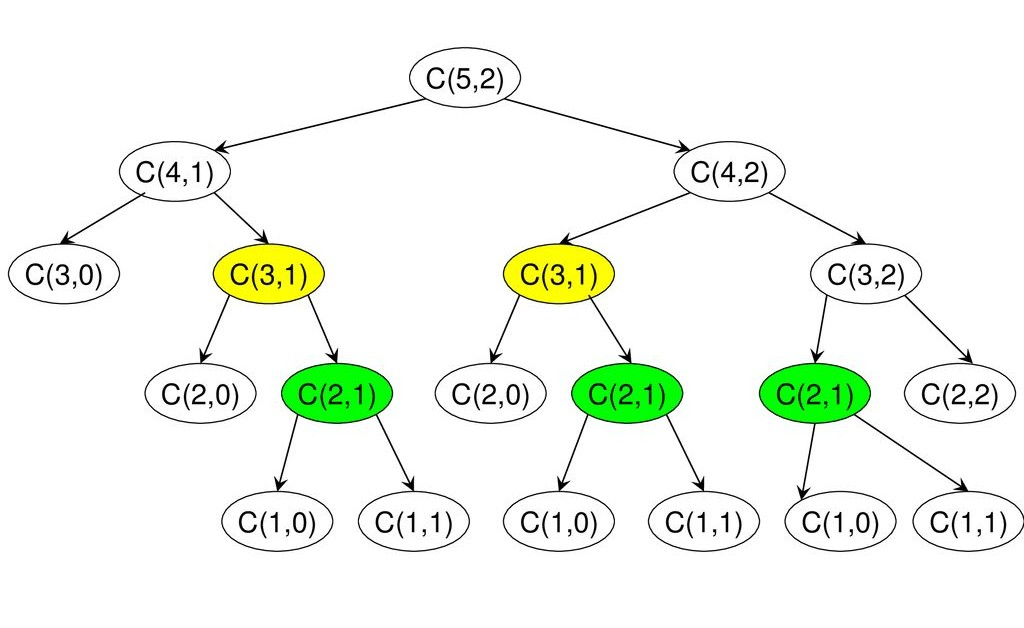
\includegraphics[width=0.8\textwidth]{combinatorio_call_tree.jpg}
    \caption*{Árbol de llamadas de \proc{Combinatorio} para la instancia $n=5, k=2$}
\end{figure}

Acá es donde entra en juego la programación dinámica. El siguiente algoritmo bottom-up calcula una única vez cada coeficiente necesario:
\begin{codebox}
    \Procname{$\proc{Combinatorio-PD}(n, k)$}
    \li Inicializar matriz $A \in \N^{n \times k}$
    \li \For $i \gets 1$ \To $n$ \Do
    \li $A[i][0] \gets 1$
    \End
    \li \For $j \gets 0$ \To $k$ \Do
    \li $A[j][j] \gets 1$
    \End
    \li \For $i \gets 2$ \To $n$ \Do
    \li \For $j \gets 2$ \To $\min{\{i - 1, k\}}$ \Do
    \li $A[i][j] \gets A[i - 1][j - 1] + A[i - 1][j]$
    \End
    \End
\end{codebox}

La complejidad de este método es\BigO{nk}, y $\BigO{nk} \subseteq \BigO{n^2}$, ya que $k \leq n$. Además, se puede implementar con una complejidad espacial de\BigO{k} almacenando solo la fila actual y la anterior de la tabla en el ciclo.

\subsection{Principio de optimalidad de Bellman}
\label{optimalidad-bellman}

Un problema satisface el \textit{principio de optimalidad de Bellman} cuando para cualquier \textit{sucesión óptima} de decisiones, cada \textit{subsucesión} es a su vez óptima para el subproblema asociado. Esta es una condición necesaria para que aplicar PD sea eficiente.

\subsubsection{Ejemplo: Problema de la mochila}
\label{problema-mochila}

\begin{problema}
    Dados
    \begin{itemize}
        \item Capacidad $C \in \Z_+$ de la mochila (peso máximo).
        \item Cantidad $n \in \Z_+$ de objetos.
        \item Peso $p_i \in \Z_+$ del objeto $i$.
        \item Beneficio $b_i \in \Z_+$ del objeto $i$.
    \end{itemize}

    Determinar qué objetos se deben incluir en la mochila para \textbf{maximizar} el beneficio total, sin \textbf{excederse} del peso máximo $C$. Formalmente, encontrar:
    $$\arg\max{\left\{\sum_{s \in S} b_s \mid S \subseteq \{1, ..., n\},\ \sum_{s \in S} p_s \leq C \right\}}$$
\end{problema}

Para resolver este problema utilizando PD, se puede definir la función $m(k, D)$ como el valor óptimo para el problema considerando solo los primeros $k$ objetos y una mochila con capacidad $D$. Los valores de esta función pueden ser guardados en una tabla de $n \times C$ posiciones. Los valores se pueden calcular de manera recursiva:
$$
    m(k, D) =
    \begin{cases}
        0                                              & \si k = 0 \lor D \leq 0 \\
        \max{\{m(k - 1, D), b_k + m(k - 1, D - p_k)\}} & \ecc
    \end{cases}
$$

Esto contempla, para cada $k$ dos posibilidades: o bien el objeto de índice $k$ está en la solución óptima, y entonces $m(k, D) = b_k + m(k - 1, D - p_k)$, o bien no, en cuyo caso $m(k, D) = m(k - 1, D)$.

Si esta función se implementa directamente en un algoritmo de PD (ya sea top-down o bottom-up) utilizando una matriz como estructura de memoización, tanto la complejidad temporal como la espacial son\BigO{nC}. Esta complejidad es \textit{pseudopolinomial}: está acotada por un polinomio, pero este incluye valores númericos del input, no solo el tamaño del mismo.

\subsubsection{Solución óptima}
\label{reconstruccion-solucion}

Calcular $m(k, D)$ nos da el \textit{valor óptimo}, pero no la \textit{solución óptima}. Para obtener el conjunto de objetos que resulta en ese valor se debe reconstruir a partir de la tabla calculada. El esquema general para la reconstrucción se basa en la observación anterior: recorriendo los índices de atrás para adelante, si $m(k, D) = b_k + m(k - 1, D - p_k)$, entonces el valor $k$ está en (alguna) solución. Si no, es porque $m(k - 1, D) > b_k + m(k - 1, D - p_k)$, es decir, ignorar el objeto $k$ resulta en un mayor beneficio total. Este procedimiento permite obtener el conjunto solución en tiempo lineal (una vez que ya se ejecutó el algoritmo anterior).

\subsubsection{Ejemplo: Multiplicación de matrices}

\begin{problema}
    Dadas $M_1, M_2, ..., M_n$, calcular:
    $$M = M_1 \times M_2 \times ... \times M_n$$

    Realizando la menor cantidad de multiplicaciones entre números de punto flotante.
\end{problema}

La dificultad de este problema radica en que la cantidad de operaciones realizadas depende de la forma en la que se asocie el producto. Para resolverlo, se puede observar que alguna de las multiplicaciones tiene que ser la última realizada, es decir, para algún $i$, se deben multiplicar primero las matrices de $1$ a $i$ por un lado y las de $i + 1$ a $n$ por el otro, y finalmente multiplicar estos $2$ resultados. Estos dos sub-problemas ($M_1 \times M_2 \times ... \times M_i$ y $M_{i+1} \times M_{i+2}\times ... \times M_n$) deben ser resueltos, a su vez, de forma óptima.

Luego, suponiendo que las dimensiones de las matrices están dadas por un vector $d \in \N^{n+1}$ tal que $M_i \in \R^{d[i-1] \times d[i]}$, se puede implementar el siguiente algoritmo bottom-up:

\begin{codebox}
    \Procname{$\proc{Min-Operaciones}(d)$}
    \li Inicializar la matriz $m \in \N^{n \times n}$
    \li \For $i \gets 1$ \To $n$ \Do
    \li $m[i][i] \gets 0$
    \End
    \li \For $i \gets 1$ \To $n - 1$ \Do
    \li $m[i][i + 1] \gets d[i - 1]d[i]d[i + 1]$
    \End
    \li \For $s \gets 2$ \To $n - 2$ \Do
    \li \For $i \gets 1$ \To $n - s$ \Do
    \li $m[i][i + s] \gets \min{\{m[i][k] + m[k+1][i+s] + d[i-1]d[k]d[i+s] \mid i \leq k < i + s\}}$
    \End
    \End
\end{codebox}

En este caso, $m[i][j]$ representa la cantidad mínima de operaciones necesarias para calcular $M_i \times M_{i+1} \times ... \times M_j$, y por ende el valor óptimo es $m[1][n]$. Para obtener la secuencia de multiplicaciones, se puede emplear un procedimiento similar \hyperref[reconstruccion-solucion]{al del ejemplo anterior}.

% TODO: Subsecuencia común más larga

\section{Algoritmos Golosos}

\subsection{Heurísticas}

Una \textit{heurística} para un problema dado es un procedimiento computacional que intenta obtener soluciones de ``buena calidad'' para el mismo. Por ejemplo, para un problema de optimización, una heurística obtendría una solución con un valor cercano al óptimo.

Un algoritmo $A$ es $\epsilon$-aproximado cuando:
$$\left|\frac{x_A - x^*}{x^*}\right| \leq \epsilon$$

Donde $x^*$ es el valor óptimo, y $x_A$ es el resultado del algoritmo.

Un ejemplo práctico es el algoritmo de Christofides y Serdykuov, un algoritmo $\frac{1}{2}$-aproximado para instancias del problema del viajante de comercio que forman un espacio métrico (las distancias son simétricas y obedecen la desigualdad triangular). Lo notable de este algoritmo es que tiene complejidad polinómica, siendo el TSP un problema NP-Completo.

\subsection{Algoritmos golosos}

Los \textit{algoritmos golosos} se basan en construir una solución para un problema seleccionando en cada la ``mejor'' alternativa, sin considerar (o haciéndolo débilmente) las implicancias posteriores de esa selección. Habitualmente, proporcionan heurísitcas sencillas para los problemas de optimización, produciendo soluciones razonables (aunque subóptimas) en tiempos eficientes. Sin embargo, existen casos donde la solución que generan es óptima.

\subsubsection{Ejemplo: Problema de la mochila}

A pesar de haber resuelto el problema \hyperref[problema-mochila]{anteriormente}, un enfoque goloso puede proveer soluciones (subóptimas) con mayor eficiencia temporal. El esquema general es agregar a la mochila el objeto $i$ que...
\begin{enumerate}
    \item ...tenga el mayor beneficio $b_i$.
    \item ...tenga el menor peso $p_i$.
    \item ...maximice $\frac{b_i}{p_i}$ (la ``densidad'').
\end{enumerate}

Se puede demostrar que, si se corre el algoritmo goloso $2$ veces, una con el primer criterio y otra con el segundo, alguno de los resultados tiene un valor de al menos la mitad de la solución óptima. Esto hace al procedimiento un algoritmo $\frac{1}{2}$-aproximado, y se puede implementar en tiempo\BigO{n\log{n}} si se ordenan los elementos previamente (es aún más eficiente usar una colas de prioridad implementadas con heap).

Por otro lado, si cambia el problema, permitiendo poner una \underline{fracción} de cada elemento en la mochila, el algoritmo goloso que utiliza el tercer criterio devuelve soluciones óptimas.

\subsubsection{Ejemplo: Problema del cambio}

\begin{problema}
    Dado un monto $m$ y un conjunto de denominaciones $d_1, ..., d_k$, encontrar la mínima cantidad de monedas necesarias para obtener el valor $m$.
\end{problema}

Para encontrar soluciones (no necesariamente óptimas) de este problema, se puede emplear un algoritmo goloso simple: en cada paso, seleccionar la moneda de mayor valor que no exceda el monto restante.

\begin{codebox}
    \Procname{$\proc{Dar-Cambio}(D, m)$}
    \li $\id{suma} \gets 0$
    \li $M \gets \{\}$
    \li \While $\id{suma} < m$ \Do
    \li $\id{pr\acute{o}xima} \gets \max{\{d \mid d \in D, d \leq m\}}$
    \li $M \gets M \cup \{\id{pr\acute{o}xima\}}$
    \li $\id{suma} \gets \id{suma} + \id{pr\acute{o}xima}$
    \End
    \li \Return $M$
\end{codebox}

Para ciertos conjuntos de denominaciones, como el tradicional ($\{1, 5, 10, 25, 50\}$), este algoritmo siempre devuelve soluciones óptimas, mientras que para otros no (en $D = \{1, 5, 10, 12\}, m = 21$, el algoritmo devuelve un conjunto de $6$ monedas cuando la solución óptima tiene $3$).

El algoritmo es goloso porque en cada paso selecciona la moneda de mayor valor posible, sin preocuparse que esto puede llevar a una mala solución, y nunca modifica una decisión tomada.

\subsubsection{Ejemplo: Tiempo de espera total en un sistema}

\begin{problema}
    Un servidor tiene $n$ clientes que puede atender en cualquier orden, y el tiempo necesario para atender al cliente $i$ es $t_i \in \R_+$. Encontrar un orden de atención que minimice el tiempo de espera total de todos los clientes.
\end{problema}

Si se denota $I = (i_1, ..., i_n)$ al orden de atención, el tiempo de espera total $T$ se puede calcular de la siguiente manera:
$$T = t_{i_1} + (t_{i_1} + t_{i_2}) + ... = \sum_{k=1}^n (n - k) t_{i_k}$$

Se puede plantear el siguiente algoritmo goloso: En cada paso, atender al cliente pendiente que tenga el menor tiempo de atención. La idea detrás de ese criterio es que el tiempo de los clientes que son atendidos primero tendrá que ser esperado por todos los demás, así que lo ideal es que sea el mínimo. Formalmente, la solución $I = (i_1, ..., i_n)$ es una que cumple $t_{i_j} \leq t_{i_{j+1}}$ para $j = 1, ..., n - 1$.

En este caso, la solución que proporciona el algoritmo resulta ser óptima. Por otro lado, la complejidad temporal es\BigO{n\log{n}}, ya que el procedimiento es equivalente a ordenar a los clientes por tiempo de espera.

\section{Algoritmos Probabilísticos}

Un \textit{algoritmo probabilístico} es uno que emplea un grado de aleatoriedad en su ejecución. Los efectos de esta aleatoriedad pueden variar: en \hyperref[las-vegas]{algunos casos} solo varía el tiempo de ejecución, mientras que \hyperref[monte-carlo]{en otros} la salida tiene una probabilidad de ser incorrecta.

\subsection{Algoritmos numéricos}

Un \textit{algoritmo numérico probabilístico} es uno que aproxima la solución a un problema matemático. Estos algoritmos suelen ser adaptaciones aleatorizadas de algoritmos clásicos, como el método de cuadratura bayesiana para la integración numérica, o el de optimización bayesiana para problemas de optimización.

\subsection{Algoritmos de Monte Carlo}
\label{monte-carlo}

Los \textit{algoritmos de Monte Carlo} son aquellos que proporcionan una respuesta que tiene cierta probabilidad (típicamente baja) de ser incorrecta. En general, si estos algoritmos se corren varias veces, la probabilidad de que la respuesta obtenida sea correcta aumenta (asumiendo independencia entre las distintas ejecuciones). Un ejemplo de estos algoritmos sería el test de primalidad de Solovay-Strassen, que siempre identifica a números primos correctamente, pero tiene una probabilidad menor a $\frac{1}{2}$ de devolver una respuesta falsa para los compuestos.

\subsection{Algoritmos de Las Vegas}
\label{las-vegas}

Los \textit{algoritmos de Las Vegas} siempre devuelven una respuesta cuando terminan, pero su tiempo de ejecución es aleatorio (potencialmente infinito). Un ejemplo podría ser un algoritmo para el problema de $n$ damas que chequea configuraciones aleatorias hasta encontrar una que satisface las restricciones.

\subsection{Algoritmos de Sherwood}

Los \textit{algoritmos de Sherwood} son algoritmos que aleatorizan procesos determinísticos, habitualmente aquellos que tienen una gran diferencia entre el peor caso y el promedio. El ejemplo clásico es el algoritmo de quicksort con pivote seleccionado aleatoriamente.
